\chapter{Test}
	\section{Introduction}
	
Dans ce chapitre, nous exposerons les différents résultats de mesures de performances obtenus par nos deux moteurs $k^2$-GraCe et P-GraCe appliqués sur plusieurs datasets dans différentes configurations. Nous commencerons par présenter l'environnement de test et les conditions d'expérimentation ainsi que les graphes utilisés et les métriques d'évaluation employés. Nous allons par la suit présenter les résultats obtenus pour chaque méthode séparément. 


	
	
	\section{Environnement de Test}
	L'environnement de test compte parmi les éléments sur lesquels repose l'optimisation de tout système. C'est un environnement permettant de tester les différentes configurations et modules. Nous présenterons dans cette partie les caractéristiques matérielles et logicielles de l'environnement de test utilisé durant nos expériences. 

	
	\begin{itemize}[label=$\bullet$]
		\item \textbf{Processeur :}
		\item \textbf{RAM : }8 GO
		\item \textbf{Cache :}
		\item \textbf{Système d'exploitation : }macOS 
		\item \textbf{Compilateur :}
	\end{itemize}
	\section{Présentation des graphes de test}
	Nous allons dans cette section présenter les graphes de tests utilisés pour l'évaluation de nos deux moteurs $k^2$-Grace et P-Grace. 
	 Le tableau \ref{graphTest} regroupe les différents graphes, la premier colonne classe les graphes selon leurs type : Statique orienté étiqueté, Statique orienté non étiqueté, Statique non orienté et Dynamique orienté. Cette diversité revient à la particularité des graphes pris en entrées et leurs caractéristiques qui différent d'une méthode à une autre.
Le tableau présente aussi les domaines d'application à partir desquels  les graphes sont issues, cette variété permettra de voir le demain pour lequel la méthode sera le plus adéquate. Les domaines que nous avons choisit sont les suivants : graphes des réseau sociaux, graphes du web et graphes bioinformatique. Le tableau donne également les caractéristiques de chaque graphe représentés par le nombre de nœuds et le nombres de liens. 
	 

	 

	\begin{table}[H]
\begin{tabular}{|l|l|l|l|l|l|l|}
\hline
\multicolumn{3}{|l|}{Type de graphe}                                                      & Graphe          & Domaine                & Nb. noeuds & Nb. liens \\ \hline
\multirow{11}{*}{\rotatebox[origin=c]{90}{ Statique } } & \multirow{7}{*}{\rotatebox[origin=c]{90}{ Orienté }} & \multirow{3}{*}{\rotatebox[origin=c]{90}{ Étiqueté}}     & ia-fb-msg       & réseaux d'interaction  & 1266       & 6451      \\ \cline{4-7} 
                           &                              &                               & tech-routers-rf & réseaux de technologie & 2113       & 6632      \\ \cline{4-7} 
                           &                              &                               & soc-hamsterster & réseaux sociaux        & 2426       & 16630     \\ \cline{3-7} 
                           &                              & \multirow{4}{*}{\rotatebox[origin=c]{90}{ Non Étiqueté }} & wiki-Vote    & réseaux de vote       & 7115 & 103689   \\ \cline{4-7} 
                           &                              &                               & soc-Slashdot   & réseaux sociaux  & 77360 & 905468   \\ \cline{4-7} 
                           &                              &                               & soc-Epinions1      & réseaux sociaux    & 75879       & 508837    \\ \cline{4-7} 
                           &                              &                               & Amazon0302      & réseaux de commerce    & 262111     & 1234877   \\ \cline{2-7} 
                           & \multicolumn{2}{l|}{\multirow{4}{*}{\rotatebox[origin=c]{90}{ Non Orienté }}}                & caida           & réseaux informatiques &			26475	 & 53381              \\ \cline{4-7} 
                           & \multicolumn{2}{l|}{}                                        &         California & 	Infrastructure	&		1,965,206 &	2,766,607     \\ \cline{4-7} 
                           & \multicolumn{2}{l|}{}                                        &           DBLP coauthorship	& Co-authorship			&317,08&	1,049,866     \\ \cline{4-7} 
                           & \multicolumn{2}{l|}{}                                        &             Brightlike &	Social Network		&	58,228 & 	214078   \\ \hline
\multirow{3}{*}{\rotatebox[origin=c]{90}{ Dynamique } } & \multicolumn{2}{l|}{\multirow{3}{*}{\rotatebox[origin=c]{90}{ Orienté }}}                &     FB-FORUM            &                       réseaux sociaux                  &      899      &   33700        \\ \cline{4-7} 
                           & \multicolumn{2}{l|}{}                                        &      fb-messages         &    réseaux sociaux     &    11900   &     59800    \\ \cline{4-7} 
                           & \multicolumn{2}{l|}{}                                        &      ia-enron-employees          &    réseaux sociaux               &      150      &         168.5 \\ \hline

\end{tabular}
\label{graphTest}
\end{table}
	
	
	\section{Évaluation du moteur $k^2$-GraCE}
	Nous allons dans cette partie présenter une évaluation des méthodes du moteur $K^2$-Grace. Nous commencerons par la méthode statique où nous allons dans un premier temps nous intéresser  à l'étude de l'influence du paramètre K sur les performances, nous analyserons par la suit l'impact des différents ordres et permutations, nous finirons par une étude de l'effet du pré-traitement appliqué sur les graphes non orienté sur la qualité de compression. Nous allons ensuite étudier la méthode dynamique où nous allons discuter et comparer entre l'utilisation des captures du graphe directement ou les graphes de changements sur les résultats de la compression.
			\subsection{Analyse de l'impact du paramètre k}
			
\begin{figure}[H]
	\centering
	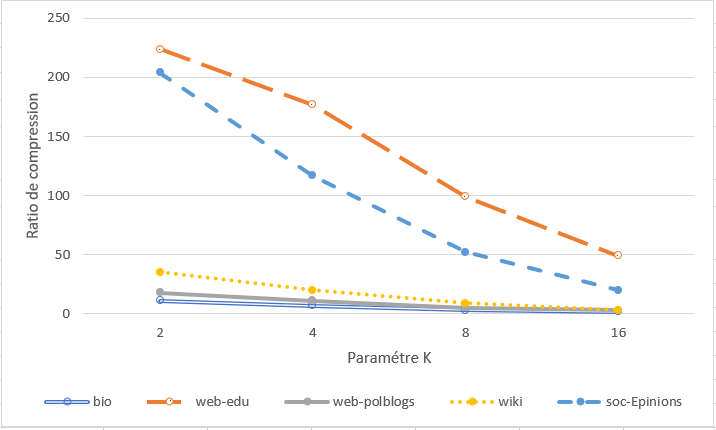
\includegraphics[scale=0.9]{ressources/image/Tests/K2-paraK-Ratio.png}
	\label{fig:K2-paraK-Ratio}
	\caption{Résultats de compression de $K^2$-Grace : Ratio de compression du moteur $K^2$-Grace en fonction du paramètre K}
\end{figure}

\begin{figure}[H]
	\centering
	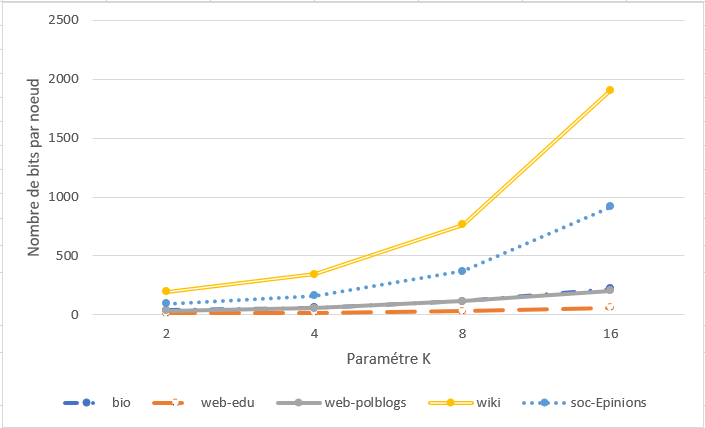
\includegraphics[scale=0.9]{ressources/image/Tests/K2-paraK-NBbits.png}
	\label{fig:K2-paraK-NBbits}
	\caption{Résultats de compression de $K^2$-Grace : Nombre de bits par nœuds en fonction du paramètre K}
\end{figure}		


Les figures \ref{fig:K2-paraK-NBbits} et\ref{fig:K2-paraK-Ratio} représentent respectivement l'évolution du nombre de bits par nœud et du ratio de compression en fonction des différentes valeurs du paramètre K. La compression a été appliquée sur différents graphes de test issues de plusieurs domaines et avec différentes caractéristiques pour avoir une meilleure analyse. Les graphes utilisés dans ce test sont : bio, web-edu, web-polblogs, wiki et soc-Epinions. Cette compression a été effectuée avec un ordre initial et sans aucun pré-traitement, avec comme paramètres :  (a voir aprés avec hafsa les noms des par). Seul le paramètre K a été varié entre 2 et 16.



D'après les résultats obtenues dans la figure \ref{fig:K2-paraK-Ratio}, nous remarquons que le ratio de compression diminue quand k prend des valeurs plus grandes et atteint sa valeur minimale (exemple : 20 pour soc-Epinions) quand K=16. Inversement, à partir de la figure \ref{fig:K2-paraK-NBbits}), nous observons que le nombre de bits par nœud augmente de manière exponentielle plus le k est grand et atteint sa valeur maximale (exemple 917 938 bits par nœud) quand K est à 16. Ainsi, nous constatons que plus le k est petit plus le ratio de compression (resp. nombre de bits par nœud) est optimal. En effet, pour des petit valeur de K, l'arbre a plus de niveaux, mais il est moins large et le nombre de ses feuilles est plus petit (petites sous matrices finales) ce qui réduit la taille de l'arbre et donne une meilleur qualité de compression. Par conséquent, plus le K est grand, plus l'arbre est remplit de feuilles et nécessite plus d'espace de stockage ce qui détériore les résultats de compression.


\begin{figure}[H]
	\centering
	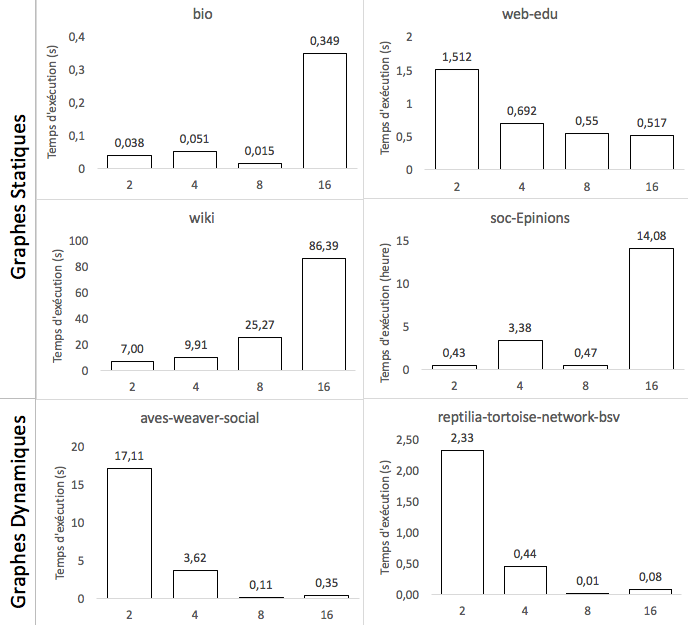
\includegraphics[scale=0.9]{ressources/image/Tests/K2-Texec.png}
	\label{fig:K2-Texec}
	\caption{Résultats de compression de $K^2$-Grace : Temps de compression en fonction de K}
\end{figure}

La figure \ref{fig:K2-Texec} représente l'évolution du temps d'exécution en fonction du paramètre K. Nous pouvons voir que le temps de compression varie de manière aléatoire et ne dépend pas de la valeur de K, ce qui est évident, car il dépend des caractéristiques du graphe (nombre de nœuds, nombre de liens, taille du fichier). 
			
			\subsection{Étude de l'effet de la représentation du graphe en entrée}
			
				\begin{figure}[H]
		\begin{center}
			\subfloat[{Bio. \label{fig:testdom2}}]
			{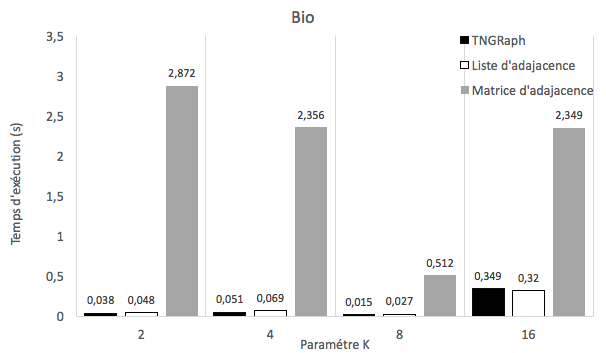
\includegraphics[width=7cm]{ressources/image/Tests/rep-bio.png}}\hspace{3em}
			\subfloat[{web-edu. \label{fig:testdom1}}]
			{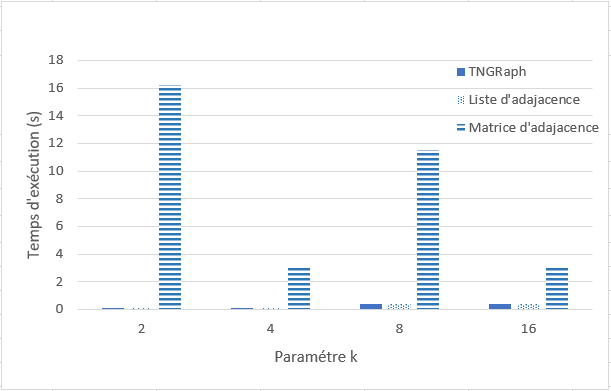
\includegraphics[width=7.5cm]{ressources/image/Tests/rep-web-edu.png}}\hspace{3em}
			\subfloat[{web-polblogs. \label{fig:testdom3}}]
			{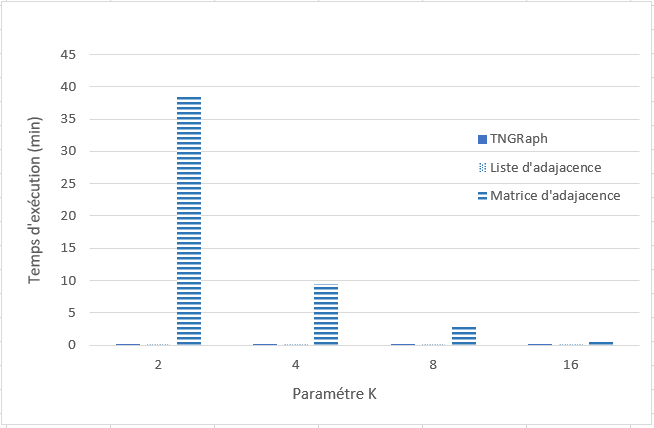
\includegraphics[width=7cm]{ressources/image/Tests/rep-web-polblogs.png}}\hspace{3em}
			
			\caption{Résultats de tests du moteur $K^2$-Grace selon les différents types de représentations du graphe en entrée.}
			\label{fig:test-rep}
		\end{center}
	\end{figure}
			
Les graphes \ref{fig:testdom1}, \ref{fig:testdom2} et \ref{fig:testdom3} représentent la variation du temps d'exécution de la méthode $k^2$-trees selon les différentes représentations du graphe en entrée appliquée sur trois graphes de tests : Bio, web-edu et web-polblogs. Cette compression a été effectuer avec un ordre initial,et avec différentes valeurs de k. 
Nous constatons d'après les trois figures que l'utilisation des trois représentations donne un temps presque égale pour les petits graphes comme Bio et edu-web. Contrairement au grandes instances où l’utilisation de la liste d’adjacence ou TNGraph donne un résultat nettement meilleur.Cela revient au temps que prend la machine pour charger la matrice d'adjacence en mémoire centrale qui devient important lorsque le graphe est grand. 
 			
\subsection{Étude de l'effet de l'ordre}

\begin{figure}[H]
	\centering
	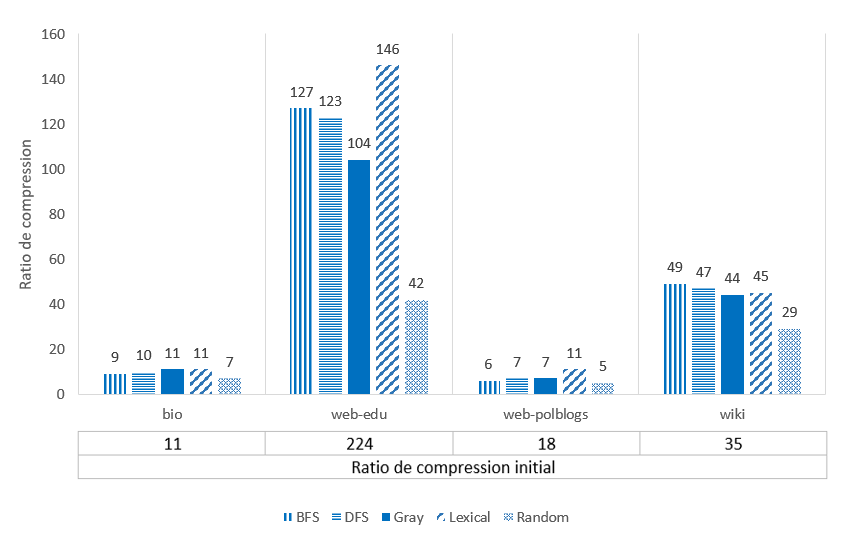
\includegraphics[scale=1]{ressources/image/Tests/k2-ordre.png}
	\label{fig:K2-ordre }
	\caption{Résultats de compression de $K^2$-Grace :Ratio de compression selon l'ordre des nœuds}
\end{figure}		

La figure \ref{fig:K2-ordre } représente l'évolution du ratio de compression du moteur $k^2$-Grace sur quatre graphes de compression : bio, web-edu, web-polblogs et wiki. Cette compression a été effectuer sur cinq ordres différents : BFS, DFS, Gray, Lexical et Random. avec comme paramètre k=2 et sans pré-traitement.
%Pas compris l amélioration a voir avec hafsa


\subsection{Étude de l'effet du pré-traitement appliqué sur les graphes statique }

Le tableau \ref{fig:tab-pret } donne les résultats de la compression du moteur $k^2$-Grace appliqué sans et avec pré-traitement sur des graphes non orientés avec un k=2 et un ordre initial de nœuds. Les graphes utilisés sont ca-netscience, Caida et Brightkite. 
Nous observons que le ratio de compression et le nombre de bits par nœud sont nettement meilleur avec le pré-traitement. Le pré-traitement appliqué sur le graphe non orienté maximise les zones vides dans la matrice d'adjacence ce qui réduit la taille de l'arbre et produit une meilleure qualité de compression. Le temps d'exécution est presque le même entre les deux exécution car le pré-traitement ne nécessite pas d'opérations couteuses en terme de temps.  

\begin{figure}[H]
	\centering
	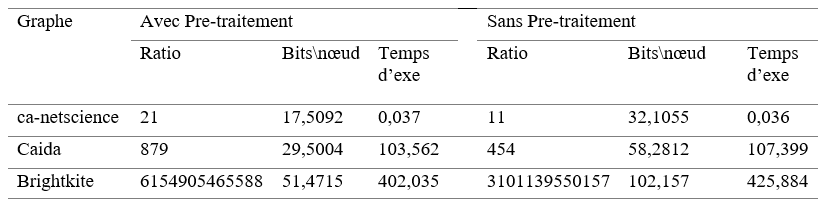
\includegraphics[scale=1]{ressources/image/Tests/tab-pret.png}
	\label{fig:tab-pret }
	\caption{Résultats de compression de $K^2$-Grace avec/sans pré-traitement}
\end{figure}


\begin{figure}[H]
	\centering
	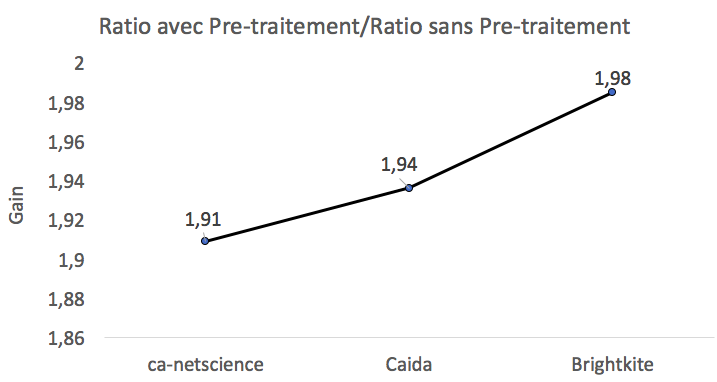
\includegraphics[scale=1]{ressources/image/Tests/gain.png}
	\label{fig:gain }
	\caption{Gain de compression de $K^2$-Grace avec le pré-traitement}
\end{figure}

La figure \ref{fig:gain } présente le gain obtenue après l'application du pré-traitement sur les graphes non orientés, nous remarquons que le gain est presque le double dans tous les graphes cela prouve que le pré-traitement améliore clairement la qualité de compression.
	\section{Évaluation du moteur P-GraCE}
	
	\section{Comparaison entre les différents moteurs}
	
	\section{Conclusion}